\providecommand{\main}{..}
\documentclass[\main/master.tex]{subfiles}
\begin{document}
\chapter{methods and results}\label{chp:example-2}
\section{vacuum system}
As explaned before when in vacuum viscous friction could be neglected. The torsional pendulum is placed inside a vacuum chamber, so the rotation angle is measured at vacuum.  since chamber is made from stainless steel, it's (a second) faraday cage, protecting from magnetic noise caused by measurement detectors.
\par
Vacuum chamber was manufactured using CF technology. Allowing to achieve ultra high vacuum (UHV), which would degrade to medium vacuum when pump is off. Chamber build is two cylindrical tubes placed on each other so the pendulum is inside, with three view ports in front. Sides viewports are used by the PID system to damp noises, and have a light guide before them. Center viewport is in front of the mirror placed on the pendulum and used to measure the rotation angle. The chamber has a 5 way which is connected to the vacuum engine and gauge.
\par
The angle measurement is made after the vacuum engine is disconnected from chamber by a valve, so it would not add rotation noise.






\section{torsion pendulum system}
The angle of torsion is measured using a mirror connected in front of the pendulum.This mirror is a part of an optical interferometer with which the mirror tilt could bedetermined.In order to balance the pendulum so the mirror would not be tilted, beside the tiltof the gravity field. The center of mass needs to be adjusted. The center of mass isadjusted using a mass from the back, to balance the mirror weight.The longer the wire and the smaller the wire diameter - wire torsion coefficient issmaller. Small coefficient achieves a better angle response to the gravity field. On theother hand the Small coefficient is leading to a very long time period of the pendulum,which while integrating over time would lead to very long measurements time. Alsothe wire needs to be strong enough to hold the masses without been teared down.


\section{pid operate (algoritm)}
\section{laser +aom}
\section{laser +aom +amp}
\section{arduino + led}
\doublespacing
\hspace{5 mm} This another example chapter with a working reference as see in Chapter~\ref{chp:example-1}. There I also made an example of an equation, see Eqn.~\ref{eqn:energy-mass-equivalence-relation}. We also created an example image, see Fig.~\ref{fig:sine-wave}.
\begin{figure}[htbp]
	\centering
	\fbox{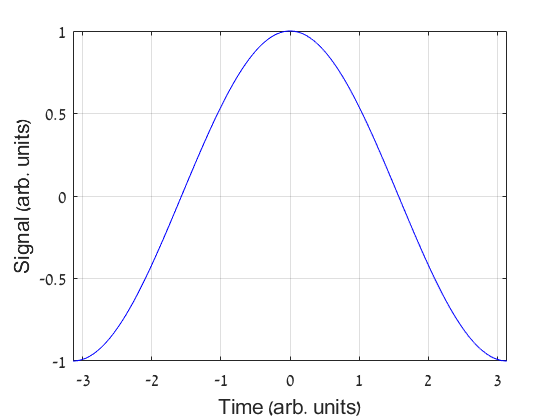
\includegraphics[scale=0.75]{\main/images/chapter_2_example/img_example_2.png}}
	\caption[Another Example Image]{Another Example Image. This image is also labeled internally so we can referenc it throughout the text.}
	\label{fig:cosine-wave}
\end{figure}
\end{document}